\documentclass[journal]{IEEEtran}

\usepackage{graphicx}
\usepackage{array}
\usepackage{subfigure}
\usepackage{adjustbox}
\usepackage{listings}
\usepackage{url}
\usepackage{cite}

\begin{document}
\title{Evolution of Processes in Delivering Reliable Software in the European Scientific Arena}

\author{E. Ronchieri,
        P. Orviz Fernandez,
        M. David,
        D. C. Duma,
        J. Gomes,
        D. Salomoni
\thanks{D. C. Duma, E. Ronchieri, and D. Salomoni are with INFN - CNAF, Bologna, Italy.}
\thanks{P. Orviz Fernandez, is with CSIC, Santander, Spain.}
\thanks{M. David, and J. Gomes are with LIP, Lisbon, Portugal.}%
}

\maketitle

\begin{abstract}

From the advent of Grid technology -- as the new paradigm of distributed
computing -- to the current days of Cloud computing models, the continuous need
of new tools and services to match the scientific community requirements has been
addressed in Europe by various projects dedicated to software development
and e--Infrastructure creation, operation and management.
This work examines the evolution of the software engineering methodologies used in past and
present European Commission--funded projects to illustrate how the research on software
reliability has progressed in Europe over the last 15 years following the foundation of the
first project in 2001. In particular, we will summarize the techniques and procedures
applied to deliver quality software, highlighting the main challenges and barriers confronted
at the time, and how they were partially or totally overcome. The knowledge base established
throughout the years, sustained by the advances in the area of software engineering,
definitely constituted a significant breakthrough in the reliability of software delivered in the
European research arena. Recent software development projects funded by the European
Commission are good evidence of such insights, where the enforcement of Quality Assurance
procedures is present since the very early stages of the software development process.

\end{abstract}

\begin{IEEEkeywords}
Software Reliability, Quality Assurance, Software Metrics, Software Testing
Techniques, DevOps
\end{IEEEkeywords}

\IEEEpeerreviewmaketitle
\section{Introduction}

\IEEEPARstart{D}{uring} the last 15 years the provision of an European e--Infrastructure,
supporting unified access to large--scale computing and intense data analysis
applications, has been driven by the needs of scientific communities as part of their
pan--European research collaborations. One such example is the Worldwide
Large Hadron Collider (LHC) Computing Grid infrastructure, driven
by the particle physics scientific community, built to satisfy the computing needs
of processing, storing and analysis of the very large amount of data produced by the
LHC particle accelerator.

A significant number of innovation projects and technology transfer
activities -- later discussed in Section~\ref{sec:ev} -- from the European Commission
(EC)-funded 5th, 6th and 7th Framework Programmes, and recently from the Horizon 2020 programme
\cite{h2020} had as their main goal to develop software solutions that provide a seamless and
transparent access by researchers to distributed computing and data resources.

Major developments carried throughout the years were focused on providing new
functionalities, whereas in the early days the adoption of software engineering methodologies had a lower priority.
The released software was less tested, resulting in a higher rate of
rollbacks and patches applied to production systems, compared to the later projects. Thereby, the stability and
% Comment
%P1 C2 L18: Claiming that stability and reliability was regularly compromised is quite a bold statement -- it needs at least some citations, and preferably some explanation of what forms this compromise took for a few prominent cases.
reliability of the e--Infrastructures was often compromised, affecting
negatively their exploitation by the scientific communities \cite{aiftimiei}.
% Comments
%P1 C2 L24: Was this realisation imposed "from above" e.g. by coordinated EC/ERC oversight, or was it "emergent" from the demands of the independent scientific communities?
It became then apparent the need for a better balance between the addition of new features
and the reliability of the released software. Consequently, incoming projects progressively
devoted a substantial part of the software lifecycle to the improvement of the quality of the
software being delivered. At this point, evolving software engineering practices were considered
and gradually adopted to define and implement quality procedures, the organization of
cross--functional teams and deployment of pilot testbeds.

Analysing the EC--funded software projects over the last decade,
one can observe a continuous increase in the prominence and robustness of software
testing and validation procedures \cite{aiftimiei}. The
evolution of the software engineering methodologies (creation of the Agile
Manifesto \cite{agile-manifesto}, and rise of DevOps practices \cite{zhu}) together
with the parallel advancements in the information and communication technology
field (such as virtualization, the enabling technology for Cloud computing and
operating--system--level virtualization known as containerization \cite{soltesz}) motivated this trend.
This evolution was complemented by the emergence of automation and event--response tools.

In this paper, we outline a set of EC--funded projects
ranging from 2001 to nowadays, in which the authors were involved.
For each project, the challenges, the methodologies and
the achievements towards software reliability are described.

The remainder of this paper is
organized as follows. Section~\ref{sec:b} summarizes the essential context of the research problem.
Section~\ref{sec:ev} details the evolution of research on
software reliability in EC--projects. Section~\ref{sec:ntsr} provides
information about new research trends in software reliability based upon the
experiences from the recent {\sl INDIGO--DataCloud} project (INDIGO--DC).
Conclusions are drawn in Section~\ref{sec:con}.

\section{Background}
\label{sec:b}

In this section, we detail the level of knowledge requested in delivering reliable software in order 
to understand the effort employed in the EC-funded software projects over time. We divide literature 
into four different domains that intersect this work: 1) software requirements, 2) software coding,
3) metrics and measurements, 4) testing.

\emph{Software requirements.} They are defined at various stages of a software development process
as a specification of what should be implemented. According to IEEE \cite{radatz}, requirement
analysis is a process for studying user needs to arrive at a definition of system, hardware or software
requirements. Characteristics of requirements that can assess software reliability are consistency and
correctness \cite{sommerville}: the former aims at providing predictable, maintainable and reliable
results, and the latter usually refers to the satisfaction of certain goals.

\emph{Software coding.} According to IEEE \cite{radatz}, coding is the process of expressing a computer
program in a programming language. To meet specific requirements, a program can be developed by using
high-level or low-level programming languages that envelope different characteristics and may affect the
result and quality of software. Furthermore, software is generally written by geographically distributed
teams whose developers can change over time, therefore it is extremely important for source code to be
understandable \cite{tashtoush}. There are various instruments that can be adopted during the software
development process to easily adapt software \cite{buse, baggen}: programming features that influence the
code readability and maintainability and standardized code that promotes the comparability of results. 

\emph{Metrics and measurements.} According to IEEE \cite{radatz}, metrics is a function, with input as 
the software data, and output is a value which could decide on how the given attribute affects the software.
Metrics and measurements have an important role in the development process \cite{fenton, capers}. Metrics
are used to improve the ability to control, identify and measure the essential parameters of software 
during its development, leading to improve the results of the software product \cite{goodman}. With a correct
usage of metrics, it is possible to determine which parts of the software require to be changed or modified.
In the literature, different types of metrics exist to be able to provide information on various software
aspects, such as complexity \cite{mccabe} and object orientation \cite{chidamber, lorenz}. Often they have 
similar definitions, so as a consequence they can be implemented in different ways according to the
interpretation of their definition. This is the reason why it has been always a challenge to select the
proper software metric tools.

\emph{Testing.} According to IEEE \cite{radatz}, testing is a process of operating a system or component
under specified conditions, observing or recording the results, and making an evaluation of some aspect of
system or component. Testing is an important factor for software quality and reliability improvement. This
activity is quite complicated due to the variety of programming languages, operating systems and hardware
platforms that evolve over time. In the current literature, there are many types of software
testing methods \cite{myers} that aim at finding errors, bugs and faults during the software development
process, possibly in the early stages. Over time, testing metrics have been defined to assess software
quality \cite{athanasiou}: code coverage is the most frequently used metric for test software reliability
and there exist many tools for dynamic code coverage estimation according to the programming language
\cite{horgan}. A dedicated effort have to be taken into account in order to integrate testing solutions
during the software development process.


\section{Evolution of research on software reliability in EC--projects}
\label{sec:ev}

The EC projects considered in this paper are listed chronologically in Table~\ref{tab:eup}.
Each project paved the way for the following ones, according to a logic evolution in which
the role of the quality and reliability of the software has
consistently increased. As shown in Table~\ref{tab:feat}, the most recent projects are more
committed to, and aware of, software reliability practices.
Table~\ref{tab:feat} also shows the topics addressed in the following sections, highlighting
the commonalities and specific features on software reliability.

\begin{table}[!h]
\renewcommand{\arraystretch}{1.3}
\caption{List of EC--projects}
\label{tab:eup}
\centering
\begin{tabular}{p{1.6cm}p{1.5cm}p{3cm}l}
\hline
\hline
\\
Logo & Short Name & Long Name & Duration\\
\hline
\hline
\begin{minipage}{.3\textwidth}

\includegraphics[width=15mm,height=7.5mm]{images/datagrid}
\end{minipage}
    & DataGrid &
Research and Technological Development for an International Data Grid & 2001--2003\\
\begin{minipage}{.3\textwidth}

\includegraphics[width=15mm,height=7.5mm]{images/egee}
\end{minipage}
     & EGEE I, II, III &
Enabling Grids for E--sciencE & 2004--2010\\
\begin{minipage}{.3\textwidth}

\includegraphics[width=15mm,height=7.5mm]{images/etics}
\end{minipage}
     & ETICS 1, 2 &
E--Infrastructure for Testing, Integration and Configuration of Software & 2006-2010\\
\begin{minipage}{.3\textwidth}

\includegraphics[width=15mm,height=7.5mm]{images/emi}
\end{minipage}
     & EMI &
Europeean Middleware Initiative & 2010--2013\\
\begin{minipage}{.3\textwidth}

\includegraphics[width=15mm,height=7.5mm]{images/egi-inspire}
\end{minipage}
     & EGI--Inspire &
Integrated Sustainable Pan--European Infrastructure for Researchers in Europe
 & 2010--2014\\
\begin{minipage}{.3\textwidth}

\includegraphics[width=15mm,height=7.5mm]{images/egi_engage}
\end{minipage}
     & EGI Engage &
Engaging the EGI Community towards an Open Science Commons
 & 2015--2017\\
\begin{minipage}{.3\textwidth}

\includegraphics[width=15mm,height=7.5mm]{images/indigo}
\end{minipage}
     & INDIGO--DataCloud &
INtegrating Distributed data Infrastructures for Global ExplOitation
 & 2015--2017\\
\hline
\hline
\end{tabular}
\end{table}

\subsection{DataGrid}

The {\sl DataGrid} \cite{cordis:datagrid} project (Jan 2001 -- Dec 2003)
main goal was to provide scientific communities, including physics, biology and
earth sciences, with intensive computing and large--scale dataset analysis capabilities.
The project brought together 21 academic and industry partners, from 15 different countries \cite{gagliardi}.
Grid was the emerging technology to be used in order to address their requirements,
thus the project delivered its own software distribution, named EDG (EU {\sl DataGrid}), strongly
based on Globus middleware components and services \cite{globus}. The project was organized in 12 work packages, from
which 5 were devoted to software development and coordinated by an
Architecture Task Force, supervising the overall design and technical consistency
of the developments.

Without previous experience in such widely
collaborative projects, a big effort was spent in devising solutions for several
challenges \cite{datagrid}, namely 1) the communication overhead, as a
result of the large geographical separation of the involved parties in the
development tasks, 2) the fast evolution of the requirements from the user
communities (50 use cases from the three scientific area), and 3) the lack of a body
of knowledge for academic software engineering.

The Agile manifesto \cite{agile-manifesto} was by then an emerging methodology, not yet
considered by the project, and as such the project's
development design suffered from the lack of the methods, tools, techniques and best
practices emerging from this new discipline of software engineering
\cite{agile}. Nevertheless, the project focused on the experiences and procedures
used by diverse collaborative open source software projects, such as Linux and Apache, trying to
achieve a higher maturity level \cite{cmm}.

\begin{table*}[!h]
\renewcommand{\arraystretch}{1.3}
\caption{Features on software reliability in EC--projects}
\label{tab:feat}
\centering
\begin{tabular}{llllllll}
\hline
\hline
Feature & DataGrid & EGEEs & ETICSs & EMI & EGIs & INDIGO--DC\\
\hline
\hline
Architecture Task Force            &$\surd$&$\surd$&$\surd$&$\surd$&$\surd$&$\surd$\\
Communication Handling             &$\surd$&$\surd$&$\surd$&$\surd$&$\surd$&$\surd$\\
Requirements Handling              &$\surd$&$\surd$&$\surd$&$\surd$&$\surd$&$\surd$\\
Agile Methodologies                &       &$\surd$&$\surd$&$\surd$&$\surd$&$\surd$\\
Source code inspection             &       &       &       &$\surd$&       &$\surd$\\
Build/Testing Management Procedure &$\surd$&$\surd$&$\surd$&$\surd$&       &$\surd$\\
Software Product Metrics           &$\surd$&$\surd$&$\surd$&$\surd$&$\surd$&$\surd$\\
Quality Criteria Definition        &       &       &$\surd$&$\surd$&$\surd$&$\surd$\\
Automatic Certification            &       &       &$\surd$&       &$\surd$&$\surd$\\
Auto--generated Documentation      &       &$\surd$&$\surd$&$\surd$&$\surd$&$\surd$\\
DevOps practices adoption (CI, CD) &       &       &       &       &       &$\surd$\\
\hline
\hline
\end{tabular}
\end{table*}

\subsection{Enabling Grids for E--sciencE}

The three phases of Enabling Grids for E--sciencE ({\sl EGEE}, Apr 2004 -- Apr 2010)
\cite{cordis:egee,cordis:egee2,cordis:egee3} projects brought together
scientists and engineers from over 240 institutions in 45 countries aiming to
provide a seamless Grid infrastructure for e--Science. {\sl EGEE--II} and {\sl EGEE--III}
featured the internationalization (outside Europe) of the project, embracing worldwide research
institutions and user communities~\cite{egee}. The software to sustain the increasing
requirements coming from the diverse scientific communities needed developing a
rich set of new services while maintaining a sustainable infrastructure for
Grid computing, eventually used by more than 15 thousand researchers and deployed in
over 250 institutions.

The {\sl gLite} middleware \cite{glite} was the
official software distribution of {\sl EGEE} as of 2006, after two years of prototyping and
re--engineering efforts to converge with the {\sl LHC} Computing Grid (LCG--2), Virtual
Data Toolkit (VDT) and Condor \cite{condor} software stacks. The
development team was comprised of more than 80 people from 12 academic and
industrial partners, which issued more than 10 thousand bug fixes, 1.7 thousand patches and
defined over 300 development tasks tracked using bug/task management tools.

The source code was available at a private, centralized version control system.
The code passed through a manual certification procedure at the time of the release.
This procedure aimed to improve the reliability of the software components by applying
acceptance criteria checks at the pre--release stage
\cite{egee:acceptance-criteria} i.e. integration, certification, pre--production and
production. Starting with {\sl EGEE--II}, the project adopted automation in the software
lifecycle process by leveraging the automatic build system for Grid middleware, that is
the {\sl ETICS} \cite{etics} solution.

\subsection{E--Infrastructure for Testing, Integration and Configuration of Software}

The E--Infrastructure for Testing, Integration and Configuration of Software~\cite{etics}
({\sl ETICS}, Jan 2006 -- Feb 2010) project aimed
at addressing the challenges in producing quality software in distributed,
collaborative projects such as {\sl EGEE} and its {\sl gLite} middleware. The framework
integrated different technologies and tools in order to provide automated configuration,
build and testing capabilities, as well as auto--generated documentation and
software metrics gathering such as Source Lines Of Code (SLOC), complexity and
number of defects/bugs \cite{etics}. The {\sl ETICS} framework was the first automated
service for delivering quality software products in distributed environments like
the Grids.

\subsection{European Middleware Initiative}

The European Middleware Initiative ({\sl EMI}, May 2010 -- Apr 2013)
\cite{cordis:emi} project joined the 4 major Grid middleware providers in
Europe at the time -- {\sl gLite}, {\sl UNICORE}, {\sl ARC} and {\sl dCache} --
with the goal to maintain and evolve the middleware focusing on extending their
interoperability and improving the reliability of the services. The
ISO/IEC 9126 \cite{iso-9126} standard was used in order to identify a set of
characteristics that needed to be present in the {\sl EMI} software products and
processes to be able to meet the {\sl EMI} quality requirements
\cite{emi-quality-model}.

For each software characteristic, a set of associated
metrics and Key Performance Indicators (KPIs) were identified and defined in
detail in the {\sl EMI} Metrics Specification \cite{emi-quality-model}. The project
leveraged the {\sl ETICS} service for the development, continuous integration and release management,
as well as for metric tracking, making queries on the collected data to display
them through the chart generation framework.

\subsection{EGI--Integrated Sustainable Pan--European Infrastructure}

The {\sl EGI--InSPIRE} (Integrated Sustainable Pan--European Infrastructure for
Researchers in Europe, May 2010 -- May 2014) project \cite{cordis:egi-inspire}
was the continuation of the {\sl EGEE--III} project, with the objective of establishing and
maintaining a sustainable European Grid Infrastructure, composed by a federation of National
Grid Initiatives and interoperable with other Grids worldwide.
This goal would be accomplished through the
development and maintenance of various operational tools, such as the Operations Portal \cite{egi-ops},
the {\sl EGI} Helpdesk \cite{ggus}, or the Grid configuration database (GOCDB) \cite{gocdb}, and the
management of the software provisioning process \cite{mario}, dealing with the validation and distribution of the software to
the production infrastructures. As a result, this process led to a production--ready
Grid computing middleware distribution named {\sl UMD} (Unified Middleware Distribution). At that time the {\sl UMD}
was a stack of about 250 software components from several technology providers, such
as {\sl EMI} and {\sl Globus}. In order to be distributed through UMD
repositories, the software had to be compliant with EGI's Quality Criteria (QC) \cite{egi-qc}. The
QC defined a set of requirements in different areas: documentation, deployment, security, information
model and operations.
{\sl UMD} is still being used and
deployed in the European scientific e--Infrastructures under the follow--up
project {\sl EGI--Engage} (Engaging the EGI Community towards an Open Science
Commons) \cite{cordis:egi-engage}. This distribution is currently complemented
by a Cloud--specific one called {\sl CMD} (Cloud Middleware Distribution).

\subsection{INtegrating Distributed data Infrastructures for Global explOitation}

The {\sl INDIGO--DataCloud} (INtegrating Distributed data Infrastructures for Global
explOitation, Apr 2015 -- Sep 2017) \cite{cordis:indigo} is the last
project of software development considered in this paper. At the time of writing,
the project is succeeding in providing solutions to address the existing gaps in
Cloud Platform--as--a--Service (PaaS) and Software--as--a--Service (SaaS) levels,
helping developers, e--Infrastructure administrators and scientific communities to exploit
Cloud computing benefits.

\section{New trends in software reliability}
\label{sec:ntsr}

{\sl INDIGO--DataCloud} is the most recent project included in this paper, it
leveraged the lessons learned from the previous experiences described in
Section~\ref{sec:ev}. The expertise gathered throughout these years was highly
profitable regarding evaluation and application of innovative software engineering
methodologies, management of new technologies to put those methodologies
into practice, compilation and analysis of an appropriate set of metrics to measure the
quality of the implemented solutions.
An additional level of complexity, comes from the fact that these large collaborative projects
have an extensive list of partners.

In the following sections, we describe the three main pillars that sustain the project's strategy to attain reliability throughout the software lifecycle:

\begin{enumerate}
    \item The definition of a \textit{Software Quality Assurance (SQA) criteria and a metrics gathering procedure} to provide guidelines
    aiming at developing quality software, validating each change in the code, to facilitate its adoption. The software lifecycle is
    continuously monitored by a set of metrics, allowing prompt reactions to detected malfunctions that may occur throughout the process. 
    \item The \textit{promotion of automation} to enable the foregoing change--based validation approach and to accelerate the delivery
    process of new software versions.
    \item A post-release validation to be carried out over the project's \textit{preview testbeds}, where the new product versions
    are deployed as part of the integration validation, and the \textit{testing in production environments} by external resource providers.
\end{enumerate}

\begin{figure}[ht]
\centering
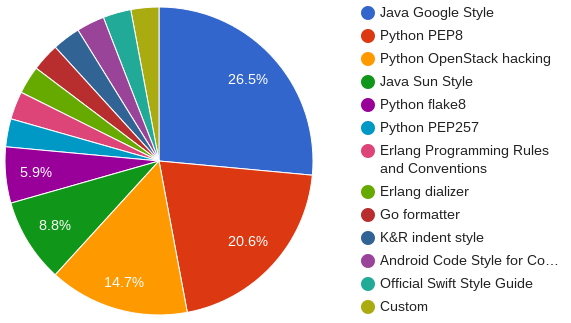
\includegraphics[width=0.5\textwidth]{images/codestyle.png}
\caption{Code style standards followed by {\sl INDIGO--DataCloud}'s software products.}
\label{fig:fig_codestyle}
\end{figure}

\begin{figure*}[ht]
\centering
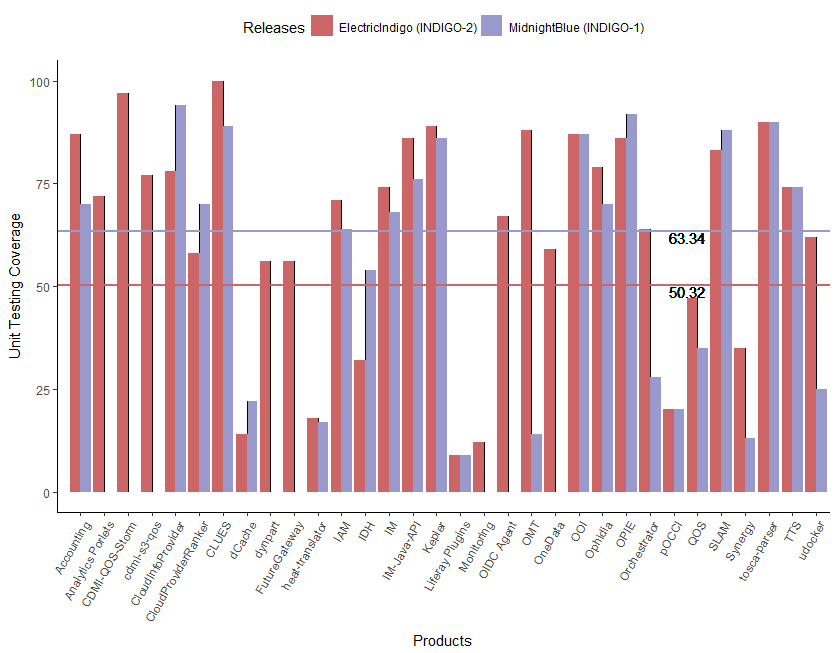
\includegraphics[width=\textwidth]{images/fig2.png}
\caption{Comparison of the unit testing coverage values for the {\sl INDIGO--DataCloud}
software stack over the {\sl INDIGO--1} and {\sl INDIGO--2} major releases.}
\label{fig:fig_unittest}
\end{figure*}

\begin{figure}[ht]
\centering
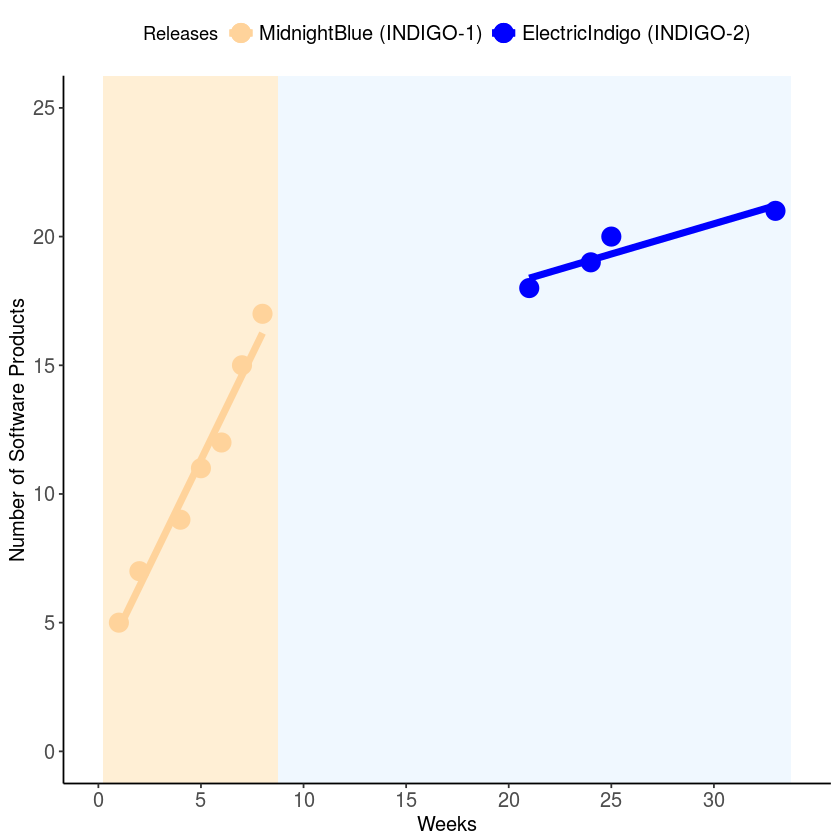
\includegraphics[width=0.5\textwidth]{images/fig3.png}
\caption{Adoption of Configuration Management tools throughout the project lifetime. Also shown the trend lines
leading to the first release (light cream points and lines), and to the second release (dark blue points and lines).}
\label{fig:fig_confman}
\end{figure}

\subsection{Software Quality Procedures}
\label{subsec:sqa}

The software quality policies were initially defined in the first deliverable document of the
project \cite{indigo-d31}. The policies were reviewed periodically taking into account the requirements
from the user communities, the feedback from the development teams and the insights of software
engineering practices. These policies covered 1) the identification
and description of the \emph{SQA requirements} that the produced software needs
to comply with, and 2) the \emph{quality metrics}, to monitor each software product's
behaviour throughout the development, release and post--release stages.

\subsubsection{SQA criteria}

The SQA criteria are a set of conventions and recommendations that pave the way for
the adequate development, timely delivery and reliable operation of the produced software components.
It emphasizes the quality requirements and best practices to be applied at the
development phase, such as style and testing compliance or human code reviews, to protect the
production source code versions. Furthermore, the criteria promote the adoption of the software
by providing minimum requirements of documentation content and stressing the usage of automated
solutions for software deployment. The SQA criteria are continuously evolving \cite{sqa-baseline}, aiming at serving
as a reference for future software development projects within the European research ecosystem.

\begin{itemize}
\item \textit{Code style}.
The ultimate goal for code style assessment is to improve the readability and reusability of the
source code produced under the scope of the
project. Code style standards are enforced for every software component in the project stack. Community
most--adopted or \textit{de--facto standards} are initially recommended, however the development teams eventually
choose the set of guidelines to comply with. Fig.~\ref{fig:fig_codestyle} highlights the code style standards and
their popularity
in the {\sl INDIGO--DataCloud} software stack.

\item \textit{Unit and Functional testing}.
Changes involving the addition of new functionalities, are required to be tested. \textit{Regression
testing} in this context is accomplished by enforcing the definition and periodic execution
of the tests, covering past fixed issues, to ensure that they are not reintroduced during the development
activities. \textit{Unit testing} completes the source code testing evaluation by focusing on the code's
internal design. The SQA criteria of {\sl INDIGO--DataCloud} set a recommended threshold of 70\% coverage
for unit testing. In Fig.~\ref{fig:fig_unittest}, unit testing coverage is compared for each software
component between the two major releases, denoting an incremental trend over the course of the project:
code coverage increased from an average value of 50.32\% to 63.34\%, outlined by the respective dates of
the project's first (INDIGO--1) and second (INDIGO--2) releases. By INDIGO--2, 53\% of the software components
(17 out of 32) were over the threshold of the aforementioned project's SQA code coverage recommendation
(70\%), while 75\% (24 out of 32) of the product stack exceeded 50\% coverage. 
The indiviual records followed also a growing trend (only 6 out of 32 components had lower values in 
INDIGO--2). It is worth noting that Fig.~\ref{fig:fig_unittest} not only includes new software developments 
implemented from scratch within the project. Software tools and libraries from 
external open--source projects -- such as {\sl tosca-parser} or {\sl heat-translator} --, contributed upstream
by the project, and well--established products, involved in {\sl INDIGO--DataCloud}
but not contributing with the 100\% of their codebases -- such as {\sl dCache} --, are also considered in the
analysis. However the values given apply to the entire codebase, even for the latter case of products. These 
products challenged the application of the SQA policies described in this section, by two means:
\begin{itemize}
    \item Previously developed code was not refactored since it was not \textit{owned} by the project.
    \item An agreement on prevailing SQA policies for such cases where quality practices were already in place.
\end{itemize}

\item \textit{Integration testing}. Software components usually interact with other services during
operation. Integration testing deals with the interactions among coupled software components or
parts of a system that cooperate to achieve a given functionality. This type of testing might be
complex and, based on the project's experience, difficult to be implemented in an automatic way. The aim is to
guarantee the overall operation of the component with regard to the services it interfaces with,
whenever new functionalities are introduced.

\item \textit{Code review}.
This phase is the last step in the change management pipeline, once the candidate change has
successfully passed through the testing methods described previously. It implies the human--based
revision of the proposed change to discuss its adequacy in terms of e.g. scope, objective fulfilment,
and documentation completeness. On approval, the candidate change is definitely merged into
the source code's production version. Human code reviewing is paramount in the software quality assessment, specially
important when the SQA testing requirements are fully automated. Secure code reviews are also
done at this stage, assessing common vulnerabilities from inputs coming from automated linters
and manual dynamic application security testing.

\item \textit{Documentation}.
The SQA criteria set the path for the adoption of the developed software by
defining the documentation content, according to the target audience. This requirement also
promotes the automation, both in terms of documentation creation and service deployment. The
\textit{documentation is treated as code}, using a markup language, automatically rendered and
uploaded to online repositories\footnote{\url{https://www.gitbook.com/@indigo-dc}}.
Thus documentation is portable and
human--reviewed, using the same workflow as the code does, validating the changes before being
updated into the production repository.

\item \textit{Automated Deployment}.
To lower the barriers of software adoption, the SQA criteria require the automated
deployment of the products delivered as part of the catalogue. Automation in this context is
tackled using a configuration management tool. These tools allow the adoption of
\textit{Infrastructure as Code} (IaC), managing the component's deployment through declarative
definitions. The definition files appear as an additional source of documentation
-- self--documenting code -- as they sequentially guide the component's deployment process on multiple
platforms. {\sl INDIGO--DataCloud} project contributed to open--source IaC tools such
as Ansible
and Puppet\footnote{\url{https://forge.puppet.com/indigodc}}. A representative example of
such contributions are the \textit{50 roles} developed from scratch and currently hosted in
the Ansible Galaxy portal\footnote{\url{https://galaxy.ansible.com/indigo-dc/}}. Fig.~\ref{fig:fig_confman}
shows the number of products that offer an automated means for deployment.
It shows an increase in the adoption of such tools leading to the {\sl INDIGO--1} release
(dark blue points and trend line), as well as to the {\sl INDIGO--2} release
(light cream points and trend line). The rate of adoption is lower during the weeks
before the second release because a significant fraction of the products had already adopted it
previously to the first release.
\end{itemize}

\subsubsection{Quality metrics}

The evaluation of the software quality is performed by measuring the values of
the metrics and Key Performance Indicators (KPIs) defined based upon the
ISO/IEC 9126 standard. These metrics cover the development, release and
maintenance phases of the software lifecycle.

\textit{Development metrics} are obtained programmatically from several sources, namely GitHub
API\footnote{\url{https://developer.github.com/v3/}.}
and Jenkins\footnote{\url{https://jenkins.io/}} service, and graphically displayed as GitHub
pages using the GrimoireLab framework\footnote{\url{http://grimoirelab.github.io/}}.
Per--component weekly reports, including the SQA requirement
fulfilment, are issued and individually discussed through the different communication channels
with the development teams. Issue tracking metrics and KPIs are an essential piece of information
of both feature addition and defect solving, useful to detect and fix misbehaviours while in the
development phase.

\textit{Release metric} sources are the online repository servers, namely the
Linux package\footnote{\url{https://jenkins.indigo-datacloud.eu/}}
and DockerHub\footnote{\url{https://hub.docker.com/u/indigodatacloud}} repositories. Jenkins
server also contains valuable release data as it is the service where the packages
and containers are being built before being uploaded to the online repositories. Release
KPIs primarily focus on the frequency and efficiency -- mainly rollbacks -- statistics.

\textit{Maintenance and user support metrics} are key for continuously improving the response
to issues reported by external users. Feedback is collected from outside helpdesks, such as
EGI's GGUS~\cite{ggus}, and the GitHub Issues tracker.

\subsection{Software quality validation and delivery automation}
\label{sec:devops}
Tackling the granularity of the former SQA requirements -- most of which accounted in a per--change basis --
is hardly achieved without the aid of automation. The introduction of automation to validate the quality
requirements increases the overall reliability of the produced software: automated testing is more 
time-efficient, leading to higher code coverages and increased defect detection, when compared with a manual
approach \cite{rafi2012}. 

As any new change, involving a new feature or fix, passes through the automated
SQA machinery, the software is always ready to be released. As a result, the often compromised harmonization
between the continouous release of new features -- pushed by the development teams -- and the maintenance of
stable production systems -- demanded by users and resource providers -- can be guaranteed. The DevOps culture
theorizes and provides practical solutions that aim at unifying both software development (dev) and software
operations (ops) teams, by emphasizing the SQA techniques to avoid infrastructure disruption whenever new
developments are deployed into production systems. 
The incremental adoption of DevOps approaches throughout the project's lifetime was a key player towards
software reliability. Starting with a CI scenario at the first stages of the project, the software delivered
was eventually validated and distributed using CD pipelines. 

\begin{figure}[ht]
\centering
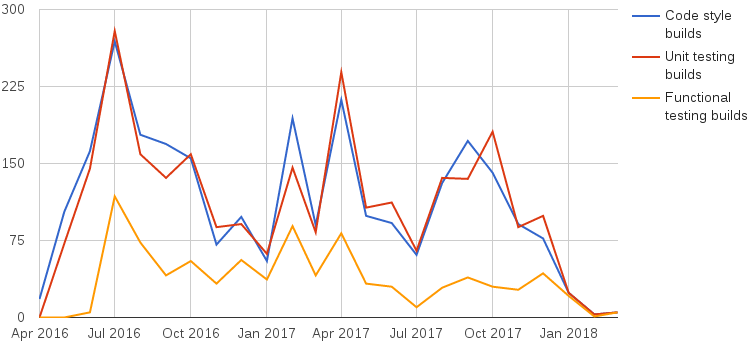
\includegraphics[width=0.5\textwidth, height=50mm]{images/jenkins_CI_builds.png}
\caption{Evolution of the total number of testing builds triggered automatically as part of the Jenkins CI implementation.}
\label{fig:fig_jenkins_CI_builds}
\end{figure}

\begin{figure*}[ht]
\centering
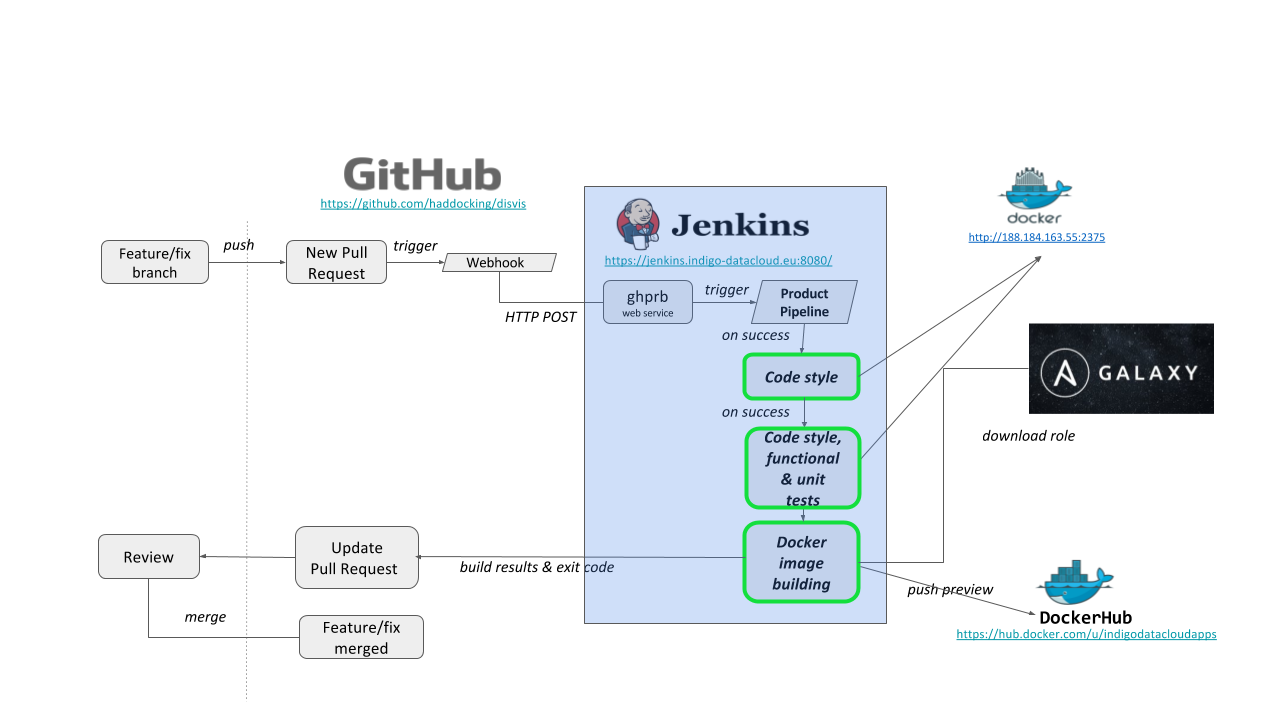
\includegraphics[width=\textwidth]{images/devops.png}
\caption{Continuous Delivery workflow for Docker images.}
\label{fig:fig_CD}
\end{figure*}


\subsubsection{Continuous Integration (CI)}
\label{subsec:ci}

The {\sl INDIGO--DataCloud} project promoted the application of a CI scenario that enforced,
for any piece of produced software, the testing requirements defined in the SQA criteria,
as described in Section \ref{subsec:sqa}. Such an environment requires an automation
ready--to--go infrastructure where the different services and technologies involved interact with each
other to trigger the source code validation pipeline for each candidate change. The
pipeline is mainly comprised by the code style validation, unit and functional testing
coverage. The CI pipeline is complemented with additional quality checks, such as
integration tests for the software components where automation of this type of testing
is applicable, or security linters for the static code analysis of suspicious
constructs that could lead to security risks. Metrics gathering is also a part of
the CI pipeline to have a per--change trend evolution of the common source code
related metrics, such as SLOC or the cyclomatic complexity.

The practical implementation of the CI scenario leverage from a tightly integrated open
source tools such as GitHub\footnote{\url{https://github.com/}}, as the online source code repository,

Jenkins is an event--response CI and Docker container
provisioning system that provides instant computing power needed for executing the pipeline jobs.
The project defined a source code contribution workflow, based on GitHub Pull Requests
(PRs), where each change automatically triggers in Jenkins the associated quality and
metric tracking checks on PR creation or update.

The CI pipeline is composed from a set of required checks, their exit status
is reported back to GitHub. The changes can be prevented if those tests are
not successfully executed.
As each change is validated, the chances
of early detection of defects increase. Within this scenario, the cost of defect solving
is dramatically reduced and the reliability of the software solutions improved, as any
bug or design issue is likely to be detected and subsequently corrected in this phase.

Fig.~\ref{fig:fig_jenkins_CI_builds} shows the evolution, throughout the
{\sl INDIGO--DataCloud}'s first and second releases, of the required test types builds since the
implementation of the CI infrastructure. Automated functional testing coverage were not
available for all the software stack, thus the associated number of builds are fewer. Towards the
end of the project, the software development activity slowed the pace but not completely ceased
as the CI infrastructure is still maintained after the project's end of life.

\subsubsection{Continuous Delivery}
As DevOps suggests, frequent releases positively affect the reliability of the software as
they reduce the time in which a given defect is exposed or has an impact, allowing the 
development teams to act promptly based on the regular feedback \cite{chen2015}. The software updates of
{\sl INDIGO--DataCloud} products, that have been taking place since the second major release, are passing through
a Continuous Delivery (CD) pipeline that adds the packaging of the software right after the
successful execution of the CI pipeline previously described. Consequently, CI--validated
software components are automatically delivered in online repositories. Nonetheless,
expert supervision to validate the results is required.

{\sl INDIGO--DataCloud} software stack is delivered in the form of Linux software packages (rpms, debs)
and Docker containers. The CD approach is different for each type of software packaging. \textit{Linux
package pipeline} intentionally delivers the packages produced in a pre--production -- preview --
branch. Before that, once the software packages have been created, they are uploaded to a
testing branch. The available automated deployment solution -- see Section \ref{subsec:sqa} -- checks
the installation and configuration of the component relying on the testing repository. On
successful completion, the packages are automatically signed and subsequently moved to
the preview branch.
In the last step, the release manager supervises the process to move the  packages to the
production branch.

The \textit{Docker container pipeline} uses the automated deployment solution to
actually install and configure the software component in the container image. Once this is
done the recently created image is uploaded to the production DockerHub repository, tagged
with the label corresponding to the current {\sl INDIGO--DataCloud} release.
Fig.~\ref{fig:fig_CD} shows the complete workflow of the Docker container CD implementation,
automatically triggered by a change in the source code.

\begin{figure*}
	\centering
	\begin{subfigure}
		\centering
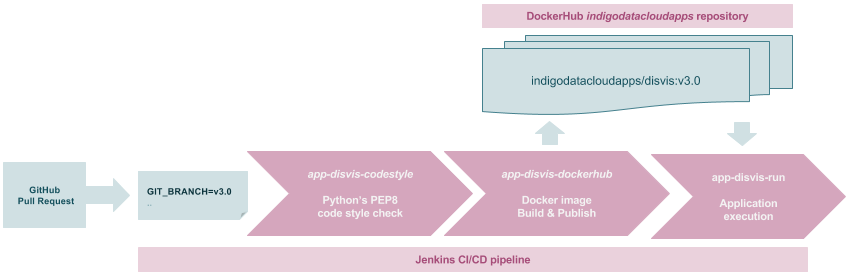
\includegraphics[width=0.85\textwidth]{images/disvis-flow.png}
\caption{DevOps pipeline to distribute Docker images for Disvis application.}
\label{fig:fig_disvis}
	\end{subfigure}
	\quad
	\begin{subfigure}
		\centering
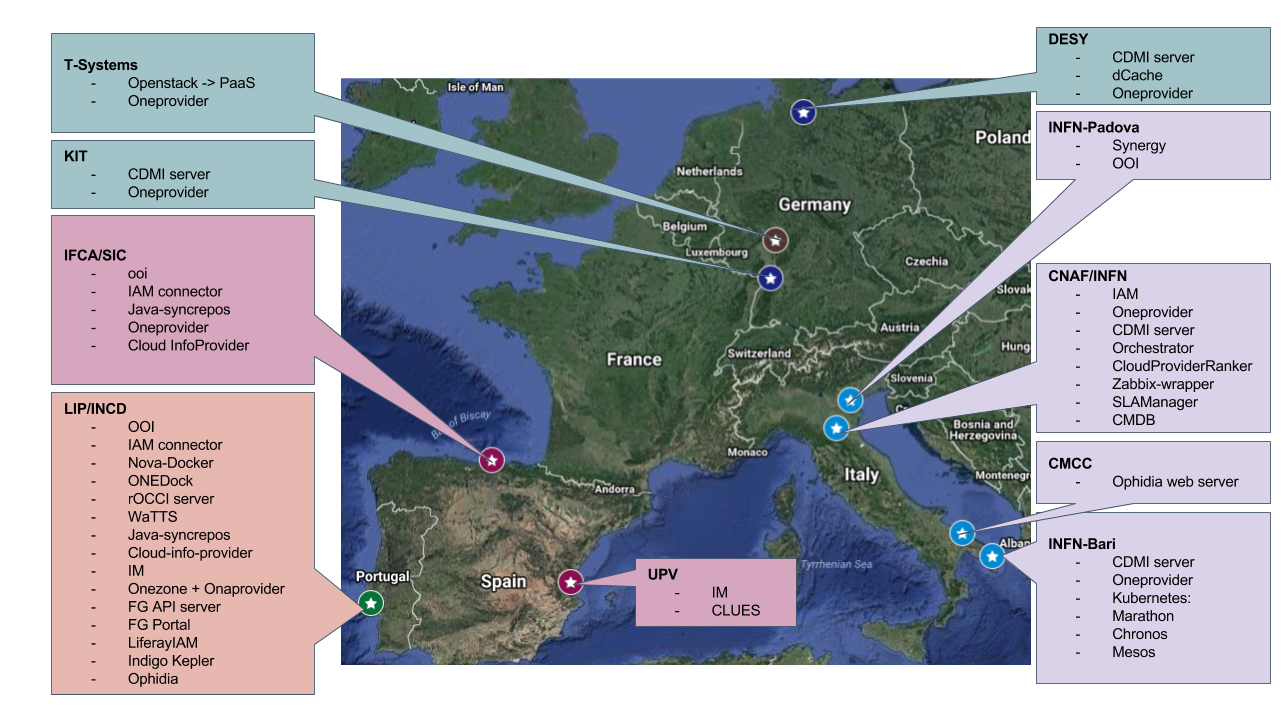
\includegraphics[width=\textwidth]{images/pilotpreview.png}
\caption{Resource centers supporting the Pilot Preview testbed and corresponding
set of deployed {\sl INDIGO--DataCloud} components or services.}
\label{fig:fig_pilotpreview}
	\end{subfigure}
\end{figure*}

\subsubsection{DevOps adoption from user communities}

The experience gathered throughout the project regarding the adoption of
different DevOps practices is not only useful and suitable for the software related
to the core services in the {\sl INDIGO--DataCloud} solution, but also applicable to the
development and distribution of the applications coming from the user communities.

Two applications from "Definition of Support to Research Communities" work package,
DisVis \cite{disvis} and PowerFit \cite{powerfit}, were
integrated into a similar CI/CD pipeline described in section \ref{sec:devops}.
Fig.~\ref{fig:fig_disvis} shows the pipeline for the Disvis application.

User application developers were provided with both a means to validate the
source code before merging and the creation of a new versioned Docker image,
automatically available in the {\sl INDIGO--DataCloud}'s application repository.

The novelty introduced in the pipeline above is the validation of the application.
Once the application is packaged as a Docker image, and subsequently uploaded
to the Dockerhub repository, it is instantiated in a new container to be validated.
The application is then executed and the results compared with a set of reference outputs.
This pipeline implementation goes a step forward by testing the application
execution for the latest available Docker image in the catalogue.

\subsection{Integration, preview and early adoption}

Two pilot infrastructures are at the disposal of developers and scientific
communities involved in the project. The aim of these testbeds is to test the
level of integration between the components involved in the {\sl INDIGO--DataCloud}
solutions and use cases validation, by deploying and executing the applications
with the last stable version of the software in environments as similar as
possible to production ones. A map of the Pilot Preview
infrastructure is depicted in Fig.~\ref{fig:fig_pilotpreview}. It shows the
resource providers and the components or services they deployed and supported.

The released software is tested in production environments through the
Staged--Rollout process, before its inclusion in the EGI's Cloud Middleware Distribution (CMD).
Selected resource providers are requested to install
the most updated stable versions of the software, and to give access to them to their users. The
Staged--Rollout process is key to detect and mitigate issues that could only
appear in production environments.

\section{Conclusion}
\label{sec:con}

After more than a decade of experiences collected throughout the reviewed
EU--funded software development and e--Infrastructure management projects, it
becomes apparent that the European software produced for scientific purposes is
evolving to a more sustainable model where the quality and reliability of
software is being prioritized. The gradual adoption of software engineering insights, such as
DevOps practices or Agile methodologies, are leading the change. In this regard, the continuous evolution of the open--source
collaborative tools, extending their capabilities to bring along tight
integrations amongst other services, matched the requirements of such practices
and procedures, facilitating in a great manner their implementation in real scenarios.

% Comment
%%P8 C1 L26: What is the demonstration that reliability has been improved significantly with the addition of stricter methologies? Is there some quantitative evidence of uptime, or bug reports per user, or similar? Or some evidence of speed of defect detection & fixing, which you cite as greatly improved? I am very sympathetic to the idea that systematic development techniques can help improve software quality (without getting into circular definitions, where "quality" means that methodologies or standards have been applied!) but there will also be a point at which the methodology gets too heavy and compromises the "agility" of the development team: how can you identify which processes are helping and which are not?
Reliability of the software has been substantially improved by applying the SQA
criteria in the development stage. Consequently, each change in the source code
that is meant to be integrated in the production version, is validated according
to the SQA testing requirements. Thus, defects are detected and corrected early in the
software lifecycle, reducing the cost of fixing errors at later stages. Automation is
key in this process, allowing the implementation of a CI scenario that enforces
the SQA criteria compliance. The application of more advanced DevOps practices
resulted in the implementation of CD pipelines to extend automation to the
delivery of packages. Thereby, safe and frequent software releases are possible, reducing
the impact on production systems. In this regard, a pre--production validation,
through the preview testbeds or resource center’s early adoption -- handled by the
Staged--rollout process -- alleviates the likelihood of discovering uncovered
issues at production.

The software lifecycle demands as well a continuous measurement and analysis
process, that allows timely reactions to discover and fix defects throughout the
development, release and maintenance stages. Conscientious metric
tracking and response sits at the core of an appropriate software maturity, as
ultimate reliability can only be achieved by enforcing and empowering the SQA
criteria through each stage of the software lifecycle.

Lessons learned show that sustainability is a key pursuit. The achievements, in terms of
processes, knowledge, software and infrastructures, shall be profited from former successful 
completed projects. In this regard, the more recent project described in this paper, {\sl INDIGO-DataCloud},
may have set the path for future reference in the European software development research ecosystem.
The SQA criteria, describing the quality requirements that might be considered during the entire
software lifecycle, have been published as open access and periodically reviewed to incorporate
new recommendations and best practices. Successful software products created during the lifetime of the 
project are maintained leveraging the same source code repositories and CI infrastructure. A seamless 
knowledge transfer among subsequent software development initiatives is key for the good progress of
delivering reliable software.


\section*{Acknowledgment}

{\sl DataGrid - Research and Technological Development for an International Data Grid}
project has received funding from the European Union's Fifth Framework Programme under
grant agreement IST--2000--25182E.

{\sl EGEE - Enabling grids For E--science} project has received funding from the European
Union's Sixth Framework Programme under grant agreement INFSO--RI--508833.

{\sl EGEE - Enabling grids For E--science--II} project has received funding from the
European Union's Sixth Framework Programme under grant agreement INFSO--RI--031688.

{\sl EGEE - Enabling grids For E--science--III} project has received funding from the
European Union's Seventh Framework Programme under grant agreement INFSO--RI--222667.

{\sl ETICS - E--Infrastructure for Testing, Integration and Configuration of Software}
project has received funding from the European Union's Sixth Framework Programme under
grant agreement INFSO--RI--026753.

{\sl ETICS - E--Infrastructure for Testing, Integration and Configuration of Software - Phase 2}
project has received funding from the European Union's Seventh Framework Programme under grant
agreement INFSO--RI--223782.

{\sl EGI--InSPIRE - European Grid Initiative: Integrated Sustainable Pan--European
Infrastructure for Researchers in Europe} project has received funding from the European
Union's Seventh Framework Programme under grant agreement INFSO--RI--261323.

{\sl EGI--Engage} project has received funding from the European Union's Horizon 2020
research and innovation programme under grant agreement RIA--654142.

{\sl INDIGO--DataCloud} project has received funding from the European Union's Horizon
2020 research and innovation programme under grant agreement RIA--653549.

\begin{thebibliography}{1}

\bibitem{h2020}
\emph{Horizon 2020} -- European Commission.
[Online] Available: \url{https://ec.europa.eu/programmes/horizon2020/}
[Accessed 4 Jun. 2018].

\bibitem{aiftimiei}
A. Aiftimiei, et al.,
Improving the quality of EMI Releases by leveraging the
EMI Testing Infrastructure.
\emph{J. Phys. Conf. Ser.},
vol. 396, 2012.

\bibitem{agile-manifesto}
K. Beck, et al., (2001),
Manifesto for Agile Software Development.
[Online] Available: \url{http://www.agilemanifesto.org/}
[Accessed 4 Jun. 2018].

\bibitem{zhu}
L. Zhu, L. Bass and G. Champlin--Scharff,
DevOps and Its Practices,
\emph{IEEE Softw.},
vol. 33, n. 3, pp. 32--34, 2016.

\bibitem{soltesz}
S. Soltesz, et. al.,
Container-based Operating System Virtualization: A Scalable, High-performance Alternative to Hypervisors,
\emph{SIGOPS Oper. Syst. Rev.},
vol. 41, n. 3, pp. 275--287, 2007.

\bibitem{radatz}
J. Radatz, A. Geraci and F. Katki,
IEEE Standard glossary of softare engineering terminology.
\emph{IEEE Std. 610.12--1990}, 1990.

\bibitem{sommerville}
I. Sommerville,
Integrated requirements engineering: A tutorial.
\emph{IEEE Softw.},
vol. 14, issue 1, pp. 16--23, 2005.

\bibitem{tashtoush}
Y. Tashtoush, et al.,
Impact of programming features on code readability.
\emph{Int. J. Softw. Eng. Appl.}, 
vol. 7, issue 6, pp. 441--458, 2013.

\bibitem{buse}
R. P. Buse and W. R. Weimer,
Learning a metric for code readability.
\emph{IEEE Trans. Softw. Eng.},
vol. 36, issue 4, pp. 546--558, 2010.

\bibitem{baggen}
R. Baggen, et al.,
Standardized code quality benchmarking for improving software maintainability.
\emph{Softw. Qual. J.},
vol. 20, issue 2, pp. 287--307, 2012.







\bibitem{fenton}
N.  Fenton,  and  S.  L.  Pfleeger.
Software  Metrics:  A  Rigorous  and  Practical Approach,
\emph{International Thomson Computer
Press}, London, UK, second edition, 1997. 

\bibitem{capers}
J. T. Capers.
Applied Software Measurement
\emph{McGrawHill}, 1991. 

\bibitem{goodman}
P. Goodman.
Practical Implementation of Software Metrics, 
\emph{McGraw Hill}, London, 1993.


\bibitem{mccabe}
T. J. McCabe.
A   Complexity   Measure,
\emph{IEEE   Transactions   on   Software Engineering},
Vol. 2, No. 4, pp. 308-320, 1976.

\bibitem{chidamber}
S.  R.  Chidamber  and  C.  E  Kemerer.
A  metrics  suite  for  Object--oriented  design,
\emph{IEEE Trans. Software Engineering}, 
June 1994.

\bibitem{lorenz}
M. Lorenz and J. Kidd.
Object-Oriented Software Metrics: A Practical Approach,
\emph{IEEE publications}.

\bibitem{myers}
G. J. Myers and C. Sandler and T. Badgett.
The art of software testing.
\emph{John Wiley \& Sons}, 2011.



\bibitem{athanasiou}
D. Athanasiou and A. Nugroho and J. Visser and A. Zaidman.
Test code quality and its relation to issue handling performance.
\emph{IEEE Transactions on Software Engineering}, 
vol. 40, issue 7, pp. 1100--1125, 2014.



\bibitem{horgan}
J. R. Horgan and S. London and M. R. Lyu.
Achieving software quality with testing coverage measuring.
\emph{IEEE Computer},
vol. 27, issue 9, pp. 60--69, 1994.



\bibitem{cordis:datagrid}
P. Kunszt,
European DataGrid project: status and plans,
\emph{Nucl. Instr. Meth. Phys. Res. A},
vol. 502, n. 2, pp. 376--381, 2003.

\bibitem{gagliardi}
Gagliardi F., Jones B., Reale M., Burke S.,
European DataGrid Project: Experiences of Deploying a Large Scale Testbed for E--science Applications,
in \emph{Performance Evaluation of Complex Systems: Techniques and Tools, LNCS},
vol. 2459, 2002.

\bibitem{globus}
I. Foster and C. Kesselman,
Globus: a Metacomputing Infrastructure Toolkit,
\emph{Int. J. Supercomput. Appl.},
vol. 11, no. 2, pp. 115--128, 1997.

\bibitem{datagrid}
L. Momtahan and A. Martin,
e--Science Experiences: Software Engineering Practice and the EU DataGrid,
in \emph{Ninth Asia--Pacific Software Engineering Conference},
pp. 269-275, 2002.

\bibitem{agile}
Torgeir Dingsoyr, Sridhar Nerur, VenuGopal Balijepally, Nils Brede Moe,
A decade of agile methodologies: Towards explaining agile software development,
\emph{J. Syst. Softw.},
vol. 85, Issue 6, pp. 1213--1221, June 2012.

\bibitem{cmm}
Paulk M., Curtis B., Chrissis M., and Weber V. C.,
Capability maturity model for software,
\emph{Software Engineering Institute},
report CMU/SEI-93-TR-24, ESC--TR-93-177, 1993.

\bibitem{cordis:egee}
\emph{Enabling Grids for E--sciencE (EGEE)} project, European Community Research and
Development Information Service (CORDIS).
[Online] Available: \url{http://cordis.europa.eu/project/rcn/80149_en.html}
[Accessed 4 Jun. 2018].

\bibitem{cordis:egee2}
\emph{Enabling Grids for E--sciencE--II (EGEE--II)} project, European Community Research and
Development Information Service (CORDIS).
[Online] Available: \url{http://cordis.europa.eu/project/rcn/99189_en.html}
[Accessed 4 Jun. 2018].

\bibitem{cordis:egee3}
\emph{Enabling Grids for E--sciencE--III (EGEE--III)} project, European Community
Research and Development Information Service (CORDIS).
[Online] Available: \url{http://cordis.europa.eu/project/rcn/87264_en.html}
[Accessed 4 Jun. 2018].

\bibitem{egee}
F. Gagliardi and M. E. B\'{e}gin,
EGEE -- providing a production quality grid for e-science,
in \emph{2005 IEEE Inter. Symp. on Mass Storage Systems and Technology},
pp. 88-92, 2005.

\bibitem{egee:acceptance-criteria}
\emph{Definition and Documentation of the Revised Software Life--Cycle Process},
Milestone MSA3.4.2, 2010, EGEE--III project.
[Online] Available: \url{https://edms.cern.ch/ui/file/1062487/2/EGEE-III-MSA3.4.2-1062487-v1_4.pdf}
[Accessed 4 Jun. 2018].

\bibitem{glite}
E. Laure et al.,
Programming the Grid with gLite,
\emph{Computational Methods in Science and Technology},
vol. 12(1), pp. 33--45, 2006.

\bibitem{condor}
D. Thain, T. Tannenbaum, M. Livny,
Condor and the Grid,
in \emph{Grid Computing: Making the Global Infrastructure a Reality},
Chapter 11, pp. 63--70, 2002.

\bibitem{etics}
A. Di Meglio, et al.,
ETICS: the international software engineering service for the grid,
in \emph{J. Phys.: Conf. Ser.},
vol. 119, n. 4, 042010, 2008.

\bibitem{cordis:emi}
C. Aiftimiei, et al.,
Towards next generations of software for distributed infrastructures: The European Middleware Initiative,
in \emph{2012 IEEE 8th Inter. Conf. on E-Science},
pp. 1--10, 2012.

\bibitem{iso-9126}
\emph{ISO/IEC 9126 Software Engineering - Product Quality},
International Organization for Standardization.
[Online] Available: \url{https://www.iso.org/standard/22749.html}
[Accessed 4 Jun. 2018].

\bibitem{emi-quality-model}
M Alandes, et al.,
Experiences with Software Quality Metrics in the EMI middleware,
in \emph{J. Phys.: Conf. Ser.}
vol. 396, n. 5, 052003, 2012.

\bibitem{cordis:egi-inspire}
I. Campos Plasencia,
EGI.eu the European grid initiative.
in \emph{4 th Iberian Grid Infrastructure Conf. Proc.},
pp. 5--15, 2010.

\bibitem{egi-ops}
H. Cordier, et al.,
From EGEE Operations Portal towards EGI Operations Portal,
in \emph{Data Driven e-Science (ISGC2010)},
pp. 129--140, 2011.

\bibitem{ggus}
T. Antoni, et al.,
Global grid user support--building a worldwide distributed user support infrastructure,
\emph{J. Phys.: Conf. Ser.},
vol. 119, n. 5, 052002, 2008.

\bibitem{gocdb}
G. Mathieu and J. Casson,
GOCDB4, a New Architecture for the European Grid Infrastructure,
in \emph{Data Driven e-Science (ISGC2010)},
pp. 163--174, 2011.

\bibitem{egi-qc}
\emph{EGI Quality Criteria}.
[Online] Available: \url{https://egi-qc.github.io/}
[Accessed 4 Jun. 2018].

\bibitem{rafi2012}
D. M. Rafi el al.,
Benefits and limitations of automated software testing: Systematic literature review and practitioner survey,
\emph{Proceedings of the 7th International Workshop on Automation of Software Test},
36--42, 2012.

\bibitem{chen2015}
L. Chen,
Continuous delivery: Huge benefits, but challenges too,
\emph{IEEE Software},
vol. 32, no 2, pp. 50--54, 2015.

\bibitem{mario}
M. David et al.,
Validation of Grid Middleware for the European Grid Infrastructure,
\emph{Journal of Grid Computing},
vol. 12, issue 3, pp. 543--558, 2014.

\bibitem{cordis:egi-engage}
\emph{Engaging the EGI Community towards an Open Science Commons (EGI--ENGAGE)}
project, European Community Research and Development Information Service (CORDIS).
[Online] Available: \url{http://cordis.europa.eu/project/rcn/194937_en.html}
[Accessed 4 Jun. 2018].

\bibitem{cordis:indigo}
Davide Salomoni, et al.,
INDIGO-DataCloud: {A} data and computing platform to facilitate seamless access to e-infrastructures,
\emph{CoRR},
vol. abs/1711.01981, 2018,
[Online] Available: \url{http://arxiv.org/abs/1711.01981}.

\bibitem{indigo-d31}
J. Gomes, et al.,
\emph{Initial Plan for WP3} INDIGO--DataCloud Deliverable 3.1.
[Online] Available: \url{https://www.indigo-datacloud.eu/documents/initial-plan-wp3-d31}
[Accessed 4 Jun. 2018].

\bibitem{sqa-baseline}
Pablo Orviz et al.,
A set of common software quality assurance baseline criteria for research projects,
2017.
[Online] Available: \url{http://digital.csic.es/bitstream/10261/160086/4/CommonSQA-v2.pdf}

\bibitem{disvis}
G.C.P. Van Zundert, A.M.J.J. Bonvin,
DisVis: quantifying and visualizing the accessible interaction space of distance
restrained biomolecular complexes,
\emph{Bioinformatics}, vol. 31, n. 19, pp. 3222--3224, 2015.

\bibitem{powerfit}
G.C.P. Van Zundert, A.M.J.J. Bonvin,
Fast and sensitive rigid--body fitting into cryo--EM density maps with PowerFit,
\emph{AIMS Biophys.}, vol. 2, n. 20150273, 73--87, 2015.

\end{thebibliography}

\end{document}
